% Options for packages loaded elsewhere
\PassOptionsToPackage{unicode}{hyperref}
\PassOptionsToPackage{hyphens}{url}
\PassOptionsToPackage{dvipsnames,svgnames,x11names}{xcolor}
%
\documentclass[
  11pt,
  letterpaper,
  DIV=11,
  numbers=noendperiod]{scrartcl}

\usepackage{amsmath,amssymb}
\usepackage{iftex}
\ifPDFTeX
  \usepackage[T1]{fontenc}
  \usepackage[utf8]{inputenc}
  \usepackage{textcomp} % provide euro and other symbols
\else % if luatex or xetex
  \usepackage{unicode-math}
  \defaultfontfeatures{Scale=MatchLowercase}
  \defaultfontfeatures[\rmfamily]{Ligatures=TeX,Scale=1}
\fi
\usepackage{lmodern}
\ifPDFTeX\else  
    % xetex/luatex font selection
\fi
% Use upquote if available, for straight quotes in verbatim environments
\IfFileExists{upquote.sty}{\usepackage{upquote}}{}
\IfFileExists{microtype.sty}{% use microtype if available
  \usepackage[]{microtype}
  \UseMicrotypeSet[protrusion]{basicmath} % disable protrusion for tt fonts
}{}
\makeatletter
\@ifundefined{KOMAClassName}{% if non-KOMA class
  \IfFileExists{parskip.sty}{%
    \usepackage{parskip}
  }{% else
    \setlength{\parindent}{0pt}
    \setlength{\parskip}{6pt plus 2pt minus 1pt}}
}{% if KOMA class
  \KOMAoptions{parskip=half}}
\makeatother
\usepackage{xcolor}
\usepackage[a4paper]{geometry}
\setlength{\emergencystretch}{3em} % prevent overfull lines
\setcounter{secnumdepth}{5}
% Make \paragraph and \subparagraph free-standing
\makeatletter
\ifx\paragraph\undefined\else
  \let\oldparagraph\paragraph
  \renewcommand{\paragraph}{
    \@ifstar
      \xxxParagraphStar
      \xxxParagraphNoStar
  }
  \newcommand{\xxxParagraphStar}[1]{\oldparagraph*{#1}\mbox{}}
  \newcommand{\xxxParagraphNoStar}[1]{\oldparagraph{#1}\mbox{}}
\fi
\ifx\subparagraph\undefined\else
  \let\oldsubparagraph\subparagraph
  \renewcommand{\subparagraph}{
    \@ifstar
      \xxxSubParagraphStar
      \xxxSubParagraphNoStar
  }
  \newcommand{\xxxSubParagraphStar}[1]{\oldsubparagraph*{#1}\mbox{}}
  \newcommand{\xxxSubParagraphNoStar}[1]{\oldsubparagraph{#1}\mbox{}}
\fi
\makeatother

\usepackage{color}
\usepackage{fancyvrb}
\newcommand{\VerbBar}{|}
\newcommand{\VERB}{\Verb[commandchars=\\\{\}]}
\DefineVerbatimEnvironment{Highlighting}{Verbatim}{commandchars=\\\{\}}
% Add ',fontsize=\small' for more characters per line
\usepackage{framed}
\definecolor{shadecolor}{RGB}{241,243,245}
\newenvironment{Shaded}{\begin{snugshade}}{\end{snugshade}}
\newcommand{\AlertTok}[1]{\textcolor[rgb]{0.68,0.00,0.00}{#1}}
\newcommand{\AnnotationTok}[1]{\textcolor[rgb]{0.37,0.37,0.37}{#1}}
\newcommand{\AttributeTok}[1]{\textcolor[rgb]{0.40,0.45,0.13}{#1}}
\newcommand{\BaseNTok}[1]{\textcolor[rgb]{0.68,0.00,0.00}{#1}}
\newcommand{\BuiltInTok}[1]{\textcolor[rgb]{0.00,0.23,0.31}{#1}}
\newcommand{\CharTok}[1]{\textcolor[rgb]{0.13,0.47,0.30}{#1}}
\newcommand{\CommentTok}[1]{\textcolor[rgb]{0.37,0.37,0.37}{#1}}
\newcommand{\CommentVarTok}[1]{\textcolor[rgb]{0.37,0.37,0.37}{\textit{#1}}}
\newcommand{\ConstantTok}[1]{\textcolor[rgb]{0.56,0.35,0.01}{#1}}
\newcommand{\ControlFlowTok}[1]{\textcolor[rgb]{0.00,0.23,0.31}{\textbf{#1}}}
\newcommand{\DataTypeTok}[1]{\textcolor[rgb]{0.68,0.00,0.00}{#1}}
\newcommand{\DecValTok}[1]{\textcolor[rgb]{0.68,0.00,0.00}{#1}}
\newcommand{\DocumentationTok}[1]{\textcolor[rgb]{0.37,0.37,0.37}{\textit{#1}}}
\newcommand{\ErrorTok}[1]{\textcolor[rgb]{0.68,0.00,0.00}{#1}}
\newcommand{\ExtensionTok}[1]{\textcolor[rgb]{0.00,0.23,0.31}{#1}}
\newcommand{\FloatTok}[1]{\textcolor[rgb]{0.68,0.00,0.00}{#1}}
\newcommand{\FunctionTok}[1]{\textcolor[rgb]{0.28,0.35,0.67}{#1}}
\newcommand{\ImportTok}[1]{\textcolor[rgb]{0.00,0.46,0.62}{#1}}
\newcommand{\InformationTok}[1]{\textcolor[rgb]{0.37,0.37,0.37}{#1}}
\newcommand{\KeywordTok}[1]{\textcolor[rgb]{0.00,0.23,0.31}{\textbf{#1}}}
\newcommand{\NormalTok}[1]{\textcolor[rgb]{0.00,0.23,0.31}{#1}}
\newcommand{\OperatorTok}[1]{\textcolor[rgb]{0.37,0.37,0.37}{#1}}
\newcommand{\OtherTok}[1]{\textcolor[rgb]{0.00,0.23,0.31}{#1}}
\newcommand{\PreprocessorTok}[1]{\textcolor[rgb]{0.68,0.00,0.00}{#1}}
\newcommand{\RegionMarkerTok}[1]{\textcolor[rgb]{0.00,0.23,0.31}{#1}}
\newcommand{\SpecialCharTok}[1]{\textcolor[rgb]{0.37,0.37,0.37}{#1}}
\newcommand{\SpecialStringTok}[1]{\textcolor[rgb]{0.13,0.47,0.30}{#1}}
\newcommand{\StringTok}[1]{\textcolor[rgb]{0.13,0.47,0.30}{#1}}
\newcommand{\VariableTok}[1]{\textcolor[rgb]{0.07,0.07,0.07}{#1}}
\newcommand{\VerbatimStringTok}[1]{\textcolor[rgb]{0.13,0.47,0.30}{#1}}
\newcommand{\WarningTok}[1]{\textcolor[rgb]{0.37,0.37,0.37}{\textit{#1}}}

\providecommand{\tightlist}{%
  \setlength{\itemsep}{0pt}\setlength{\parskip}{0pt}}\usepackage{longtable,booktabs,array}
\usepackage{calc} % for calculating minipage widths
% Correct order of tables after \paragraph or \subparagraph
\usepackage{etoolbox}
\makeatletter
\patchcmd\longtable{\par}{\if@noskipsec\mbox{}\fi\par}{}{}
\makeatother
% Allow footnotes in longtable head/foot
\IfFileExists{footnotehyper.sty}{\usepackage{footnotehyper}}{\usepackage{footnote}}
\makesavenoteenv{longtable}
\usepackage{graphicx}
\makeatletter
\def\maxwidth{\ifdim\Gin@nat@width>\linewidth\linewidth\else\Gin@nat@width\fi}
\def\maxheight{\ifdim\Gin@nat@height>\textheight\textheight\else\Gin@nat@height\fi}
\makeatother
% Scale images if necessary, so that they will not overflow the page
% margins by default, and it is still possible to overwrite the defaults
% using explicit options in \includegraphics[width, height, ...]{}
\setkeys{Gin}{width=\maxwidth,height=\maxheight,keepaspectratio}
% Set default figure placement to htbp
\makeatletter
\def\fps@figure{htbp}
\makeatother

\usepackage{fvextra} % Enhanced verbatim environment
\DefineVerbatimEnvironment{Highlighting}{Verbatim}{
  breaklines,       % Allow line breaks in long code
  commandchars=\\\{\}, % Command characters for highlighting
  fontsize=\small  % Reduce font size for better fit
}
\KOMAoption{captions}{tableheading}
\makeatletter
\@ifpackageloaded{caption}{}{\usepackage{caption}}
\AtBeginDocument{%
\ifdefined\contentsname
  \renewcommand*\contentsname{Table of contents}
\else
  \newcommand\contentsname{Table of contents}
\fi
\ifdefined\listfigurename
  \renewcommand*\listfigurename{List of Figures}
\else
  \newcommand\listfigurename{List of Figures}
\fi
\ifdefined\listtablename
  \renewcommand*\listtablename{List of Tables}
\else
  \newcommand\listtablename{List of Tables}
\fi
\ifdefined\figurename
  \renewcommand*\figurename{Figure}
\else
  \newcommand\figurename{Figure}
\fi
\ifdefined\tablename
  \renewcommand*\tablename{Table}
\else
  \newcommand\tablename{Table}
\fi
}
\@ifpackageloaded{float}{}{\usepackage{float}}
\floatstyle{ruled}
\@ifundefined{c@chapter}{\newfloat{codelisting}{h}{lop}}{\newfloat{codelisting}{h}{lop}[chapter]}
\floatname{codelisting}{Listing}
\newcommand*\listoflistings{\listof{codelisting}{List of Listings}}
\makeatother
\makeatletter
\makeatother
\makeatletter
\@ifpackageloaded{caption}{}{\usepackage{caption}}
\@ifpackageloaded{subcaption}{}{\usepackage{subcaption}}
\makeatother

\ifLuaTeX
  \usepackage{selnolig}  % disable illegal ligatures
\fi
\usepackage{bookmark}

\IfFileExists{xurl.sty}{\usepackage{xurl}}{} % add URL line breaks if available
\urlstyle{same} % disable monospaced font for URLs
\hypersetup{
  pdftitle={ML\_MP2},
  pdfauthor={Clarice Tee},
  colorlinks=true,
  linkcolor={blue},
  filecolor={Maroon},
  citecolor={Blue},
  urlcolor={Blue},
  pdfcreator={LaTeX via pandoc}}


\title{ML\_MP2}
\author{Clarice Tee}
\date{2025-02-13}

\begin{document}
\maketitle

\RecustomVerbatimEnvironment{verbatim}{Verbatim}{
  showspaces=false,
  showtabs=false,
  breaksymbolleft={},
  breaklines
}

\renewcommand*\contentsname{Table of contents}
{
\hypersetup{linkcolor=}
\setcounter{tocdepth}{3}
\tableofcontents
}

\section{Part 2}\label{part-2}

1.Beyond the factors listed in Table 1, I think that whether a firm
commits tax evasion or not will depend on many other factors, some
difficult to quantify, others hard to uncover. The listed variables will
already provide us with a valuable information that are reasons to
beliee that tax evasion has occured. These include, the company's
internal ethos, accounting transparency mechanisms, the types of
accounts/assets the company owns (e.g.~offshore/shell companies, crypto
assets), types of ``business expenses'', bribery by the
company/corruption by some government officials.

\begin{enumerate}
\def\labelenumi{\arabic{enumi}.}
\setcounter{enumi}{1}
\tightlist
\item
  In this case, KNN is better for several reasons. Firstly, it is a
  non-parametric method, thus does not need/assume a functional form for
  the relationship between X and Y variables. So, even without explicity
  interaction terms, KNN is flexible enough to identify and incorporate
  the interactions. Secondly, this means that KNN is more adaptable to
  complex patterns (non-linear). Finally, KNN uses data to predict using
  data on observatins of the nearest neighbors which are similar. So KNN
  can effectively capture the interction between predictors if it is
  important to the true relationship because it is non-parametric,
  unlike LPM. (see: 112-115 and PhoenixAI )
\end{enumerate}

\section{Part 3}\label{part-3}

\begin{Shaded}
\begin{Highlighting}[]
\ImportTok{import}\NormalTok{ pandas }\ImportTok{as}\NormalTok{ pd}
\ImportTok{import}\NormalTok{ numpy }\ImportTok{as}\NormalTok{ np}
\ImportTok{import}\NormalTok{ statsmodels.formula.api }\ImportTok{as}\NormalTok{ smf}
\ImportTok{import}\NormalTok{ seaborn }\ImportTok{as}\NormalTok{ sns}
\ImportTok{import}\NormalTok{ matplotlib.pyplot }\ImportTok{as}\NormalTok{ plt}
\ImportTok{from}\NormalTok{ matplotlib }\ImportTok{import}\NormalTok{ pyplot}
\ImportTok{import}\NormalTok{ os}
\ImportTok{import}\NormalTok{ statsmodels.formula.api }\ImportTok{as}\NormalTok{ smf}
\ImportTok{from}\NormalTok{ sklearn.preprocessing }\ImportTok{import}\NormalTok{ MinMaxScaler}
\ImportTok{from}\NormalTok{ sklearn.linear\_model }\ImportTok{import}\NormalTok{ LinearRegression}
\ImportTok{from}\NormalTok{ sklearn.linear\_model }\ImportTok{import}\NormalTok{ LinearRegression }\ImportTok{as}\NormalTok{ lm}
\ImportTok{from}\NormalTok{ sklearn.model\_selection }\ImportTok{import}\NormalTok{ train\_test\_split}
\ImportTok{from}\NormalTok{ sklearn.metrics }\ImportTok{import}\NormalTok{ mean\_absolute\_error, r2\_score, mean\_squared\_error}
\ImportTok{from}\NormalTok{ sklearn.metrics }\ImportTok{import}\NormalTok{ accuracy\_score, precision\_score, confusion\_matrix, roc\_curve, roc\_auc\_score, RocCurveDisplay}
\ImportTok{from}\NormalTok{ sklearn.neighbors }\ImportTok{import}\NormalTok{ KNeighborsClassifier}
\ImportTok{from}\NormalTok{ sklearn.model\_selection }\ImportTok{import}\NormalTok{ GridSearchCV, KFold, train\_test\_split}
\ImportTok{from}\NormalTok{ sklearn.preprocessing }\ImportTok{import}\NormalTok{ StandardScaler}
\ImportTok{from}\NormalTok{ sklearn.metrics }\ImportTok{import}\NormalTok{ precision\_score}
\ImportTok{from}\NormalTok{ sklearn.metrics }\ImportTok{import}\NormalTok{ accuracy\_score, precision\_score, confusion\_matrix, roc\_curve, roc\_auc\_score, RocCurveDisplay}
\end{Highlighting}
\end{Shaded}

\begin{Shaded}
\begin{Highlighting}[]
\CommentTok{\# Load the dataset}
\NormalTok{directory }\OperatorTok{=} \VerbatimStringTok{r"C:\textbackslash{}Users\textbackslash{}clari\textbackslash{}OneDrive\textbackslash{}Documents\textbackslash{}Machine Learning\textbackslash{}mp2"}
\NormalTok{audit\_path }\OperatorTok{=}\NormalTok{ os.path.join(directory, }\StringTok{"Data{-}Audit.csv"}\NormalTok{)}
\NormalTok{audit\_df }\OperatorTok{=}\NormalTok{ pd.read\_csv(audit\_path)}
\BuiltInTok{print}\NormalTok{(audit\_df.dtypes)}
\BuiltInTok{print}\NormalTok{(audit\_df.shape)}
\NormalTok{audit\_df.head()}
\end{Highlighting}
\end{Shaded}

\begin{verbatim}
Sector_score     float64
PARA_A           float64
Risk_A           float64
PARA_B           float64
Risk_B           float64
Money_Value      float64
Risk_D           float64
Score            float64
Inherent_Risk    float64
Audit_Risk       float64
Risk               int64
dtype: object
(776, 11)
\end{verbatim}

\begin{longtable}[]{@{}llllllllllll@{}}
\toprule\noalign{}
& Sector\_score & PARA\_A & Risk\_A & PARA\_B & Risk\_B & Money\_Value &
Risk\_D & Score & Inherent\_Risk & Audit\_Risk & Risk \\
\midrule\noalign{}
\endhead
\bottomrule\noalign{}
\endlastfoot
0 & 3.89 & 4.18 & 2.508 & 2.50 & 0.500 & 3.38 & 0.676 & 2.4 & 8.574 &
1.7148 & 1 \\
1 & 3.89 & 0.00 & 0.000 & 4.83 & 0.966 & 0.94 & 0.188 & 2.0 & 2.554 &
0.5108 & 0 \\
2 & 3.89 & 0.51 & 0.102 & 0.23 & 0.046 & 0.00 & 0.000 & 2.0 & 1.548 &
0.3096 & 0 \\
3 & 3.89 & 0.00 & 0.000 & 10.80 & 6.480 & 11.75 & 7.050 & 4.4 & 17.530 &
3.5060 & 1 \\
4 & 3.89 & 0.00 & 0.000 & 0.08 & 0.016 & 0.00 & 0.000 & 2.0 & 1.416 &
0.2832 & 0 \\
\end{longtable}

\begin{Shaded}
\begin{Highlighting}[]
\NormalTok{na\_count }\OperatorTok{=}\NormalTok{ pd.DataFrame(np.}\BuiltInTok{sum}\NormalTok{(audit\_df.isna(), axis }\OperatorTok{=} \DecValTok{0}\NormalTok{), columns }\OperatorTok{=}\NormalTok{ [}\StringTok{"Count NAs"}\NormalTok{])}
\BuiltInTok{print}\NormalTok{(na\_count)}
\NormalTok{audit\_df }\OperatorTok{=}\NormalTok{ audit\_df.dropna()}
\end{Highlighting}
\end{Shaded}

\begin{verbatim}
               Count NAs
Sector_score           0
PARA_A                 0
Risk_A                 0
PARA_B                 0
Risk_B                 0
Money_Value            1
Risk_D                 0
Score                  0
Inherent_Risk          0
Audit_Risk             0
Risk                   0
\end{verbatim}

\begin{Shaded}
\begin{Highlighting}[]
\CommentTok{\# Sort our target and features into different dataframes}
\NormalTok{X }\OperatorTok{=}\NormalTok{ audit\_df.drop([}\StringTok{\textquotesingle{}Risk\textquotesingle{}}\NormalTok{], axis }\OperatorTok{=} \DecValTok{1}\NormalTok{)}
\NormalTok{target }\OperatorTok{=}\NormalTok{ audit\_df.loc[:,}\StringTok{\textquotesingle{}Risk\textquotesingle{}}\NormalTok{]}
\NormalTok{display(X.head())}
\NormalTok{display(target.head())}

\NormalTok{target.value\_counts()}

\CommentTok{\# Split training/validation set}
\NormalTok{X\_train, X\_valid, target\_train, target\_valid }\OperatorTok{=}\NormalTok{ train\_test\_split(}
\NormalTok{X, target, train\_size}\OperatorTok{=}\FloatTok{0.50}\NormalTok{, random\_state}\OperatorTok{=}\DecValTok{13}
\NormalTok{)}
\end{Highlighting}
\end{Shaded}

\begin{longtable}[]{@{}lllllllllll@{}}
\toprule\noalign{}
& Sector\_score & PARA\_A & Risk\_A & PARA\_B & Risk\_B & Money\_Value &
Risk\_D & Score & Inherent\_Risk & Audit\_Risk \\
\midrule\noalign{}
\endhead
\bottomrule\noalign{}
\endlastfoot
0 & 3.89 & 4.18 & 2.508 & 2.50 & 0.500 & 3.38 & 0.676 & 2.4 & 8.574 &
1.7148 \\
1 & 3.89 & 0.00 & 0.000 & 4.83 & 0.966 & 0.94 & 0.188 & 2.0 & 2.554 &
0.5108 \\
2 & 3.89 & 0.51 & 0.102 & 0.23 & 0.046 & 0.00 & 0.000 & 2.0 & 1.548 &
0.3096 \\
3 & 3.89 & 0.00 & 0.000 & 10.80 & 6.480 & 11.75 & 7.050 & 4.4 & 17.530 &
3.5060 \\
4 & 3.89 & 0.00 & 0.000 & 0.08 & 0.016 & 0.00 & 0.000 & 2.0 & 1.416 &
0.2832 \\
\end{longtable}

\begin{verbatim}
0    1
1    0
2    0
3    1
4    0
Name: Risk, dtype: int64
\end{verbatim}

LPM

\begin{Shaded}
\begin{Highlighting}[]
\CommentTok{\# Fit the model}
\NormalTok{lpm}\OperatorTok{=}\NormalTok{lm().fit(X\_train, target\_train)}
\CommentTok{\# Apply the model to the validation set}
\NormalTok{lpm\_pred }\OperatorTok{=}\NormalTok{ lpm.predict(X\_valid)}
\end{Highlighting}
\end{Shaded}

3.a. For firms with a predicted probability of tax evasion greater than
0:5, construct the confusion matrix.

\begin{Shaded}
\begin{Highlighting}[]
\NormalTok{lpm\_pred\_5 }\OperatorTok{=}\NormalTok{ np.where(lpm\_pred }\OperatorTok{\textgreater{}} \FloatTok{0.5}\NormalTok{, }\DecValTok{1}\NormalTok{, }\DecValTok{0}\NormalTok{)}

\CommentTok{\# Confusion matrix}
\NormalTok{lmp\_cm\_5 }\OperatorTok{=}\NormalTok{ confusion\_matrix(target\_valid, lpm\_pred\_5, normalize}\OperatorTok{=}\StringTok{"true"}\NormalTok{)}
\CommentTok{\# Display the visualization of the confusion matrix}
\NormalTok{fig, ax }\OperatorTok{=}\NormalTok{ plt.subplots(figsize}\OperatorTok{=}\NormalTok{(}\DecValTok{9}\NormalTok{, }\DecValTok{9}\NormalTok{))}
\NormalTok{ax }\OperatorTok{=}\NormalTok{ sns.heatmap(}
\NormalTok{lmp\_cm\_5, annot}\OperatorTok{=}\VariableTok{True}\NormalTok{, fmt}\OperatorTok{=}\StringTok{".2\%"}\NormalTok{, cmap}\OperatorTok{=}\StringTok{"Blues"}
\NormalTok{)}
\NormalTok{ax.set\_title(}\StringTok{"LPM: Confusion Matrix with targets (threshold of 0.5)}\CharTok{\textbackslash{}n}\StringTok{"}\NormalTok{)}
\NormalTok{ax.set\_xlabel(}\StringTok{"}\CharTok{\textbackslash{}n}\StringTok{Predicted Values (threshold of 0.5)"}\NormalTok{)}
\NormalTok{ax.set\_ylabel(}\StringTok{"Actual Values"}\NormalTok{)}
\NormalTok{ax.xaxis.set\_ticklabels([}\StringTok{"False"}\NormalTok{, }\StringTok{"True"}\NormalTok{])}
\NormalTok{ax.yaxis.set\_ticklabels([}\StringTok{"False"}\NormalTok{, }\StringTok{"True"}\NormalTok{])}
\NormalTok{plt.show()}
\end{Highlighting}
\end{Shaded}

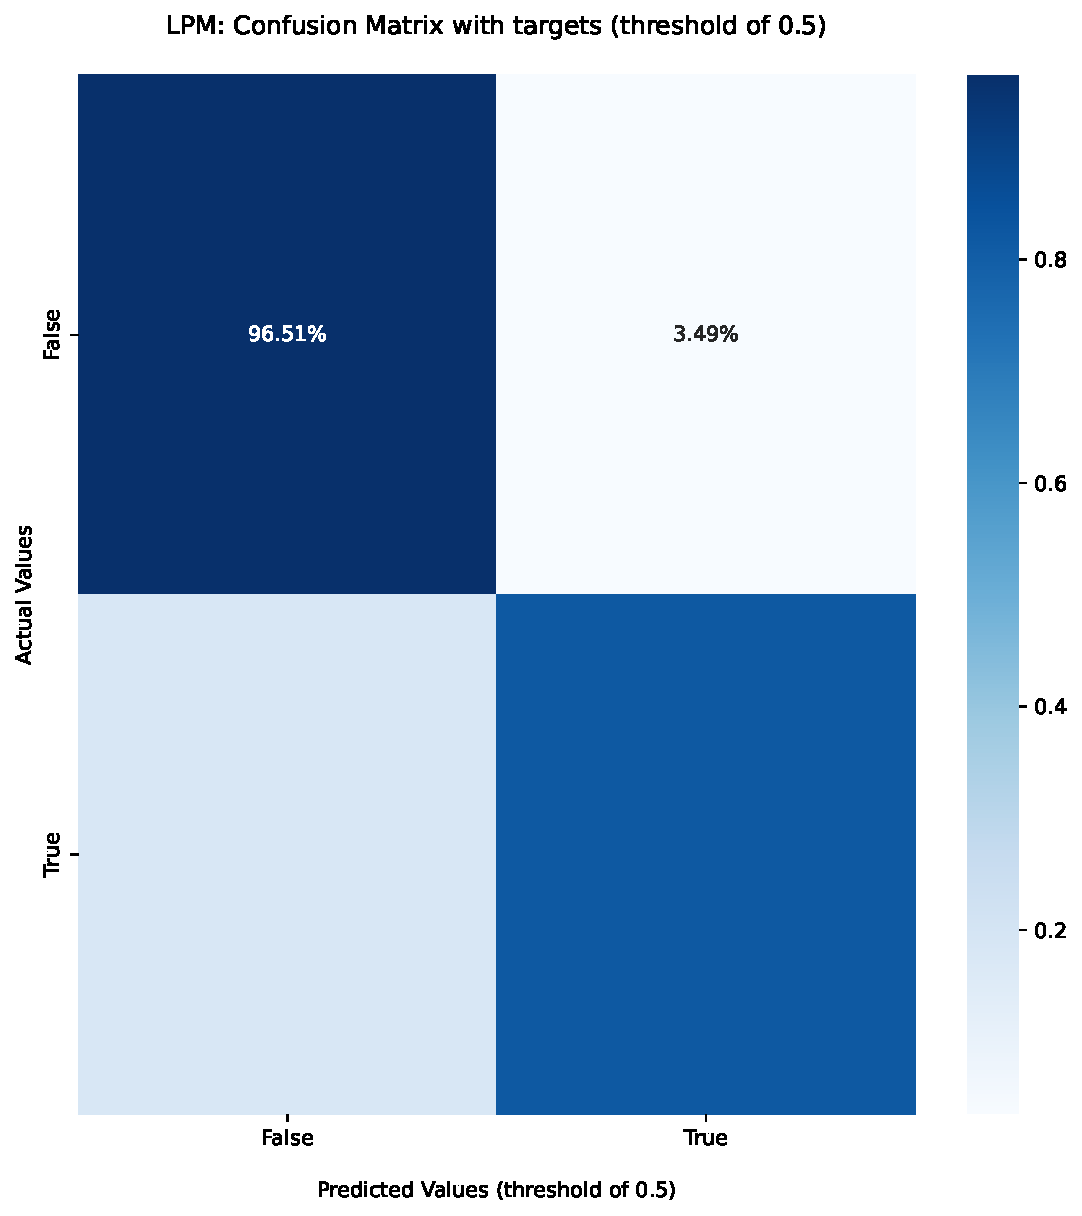
\includegraphics{mp2_files/figure-pdf/cell-7-output-1.pdf}

3.b.

\begin{Shaded}
\begin{Highlighting}[]
\NormalTok{lpm\_pred\_6 }\OperatorTok{=}\NormalTok{ np.where(lpm\_pred }\OperatorTok{\textgreater{}} \FloatTok{0.6}\NormalTok{, }\DecValTok{1}\NormalTok{, }\DecValTok{0}\NormalTok{)}

\CommentTok{\# Confusion matrix}
\NormalTok{lmp\_cm\_6 }\OperatorTok{=}\NormalTok{ confusion\_matrix(target\_valid, lpm\_pred\_6, normalize}\OperatorTok{=}\StringTok{"true"}\NormalTok{)}
\CommentTok{\# Display the visualization of the confusion matrix}
\NormalTok{fig, ax }\OperatorTok{=}\NormalTok{ plt.subplots(figsize}\OperatorTok{=}\NormalTok{(}\DecValTok{9}\NormalTok{, }\DecValTok{9}\NormalTok{))}
\NormalTok{ax }\OperatorTok{=}\NormalTok{ sns.heatmap(}
\NormalTok{lmp\_cm\_6, annot}\OperatorTok{=}\VariableTok{True}\NormalTok{, fmt}\OperatorTok{=}\StringTok{".2\%"}\NormalTok{, cmap}\OperatorTok{=}\StringTok{"Blues"}
\NormalTok{)}
\NormalTok{ax.set\_title(}\StringTok{"LPM: Confusion Matrix with targets (threshold of 0.6)}\CharTok{\textbackslash{}n}\StringTok{"}\NormalTok{)}
\NormalTok{ax.set\_xlabel(}\StringTok{"}\CharTok{\textbackslash{}n}\StringTok{Predicted Values (threshold of 0.6)"}\NormalTok{)}
\NormalTok{ax.set\_ylabel(}\StringTok{"Actual Values"}\NormalTok{)}
\NormalTok{ax.xaxis.set\_ticklabels([}\StringTok{"False"}\NormalTok{, }\StringTok{"True"}\NormalTok{])}
\NormalTok{ax.yaxis.set\_ticklabels([}\StringTok{"False"}\NormalTok{, }\StringTok{"True"}\NormalTok{])}
\NormalTok{plt.show()}
\end{Highlighting}
\end{Shaded}

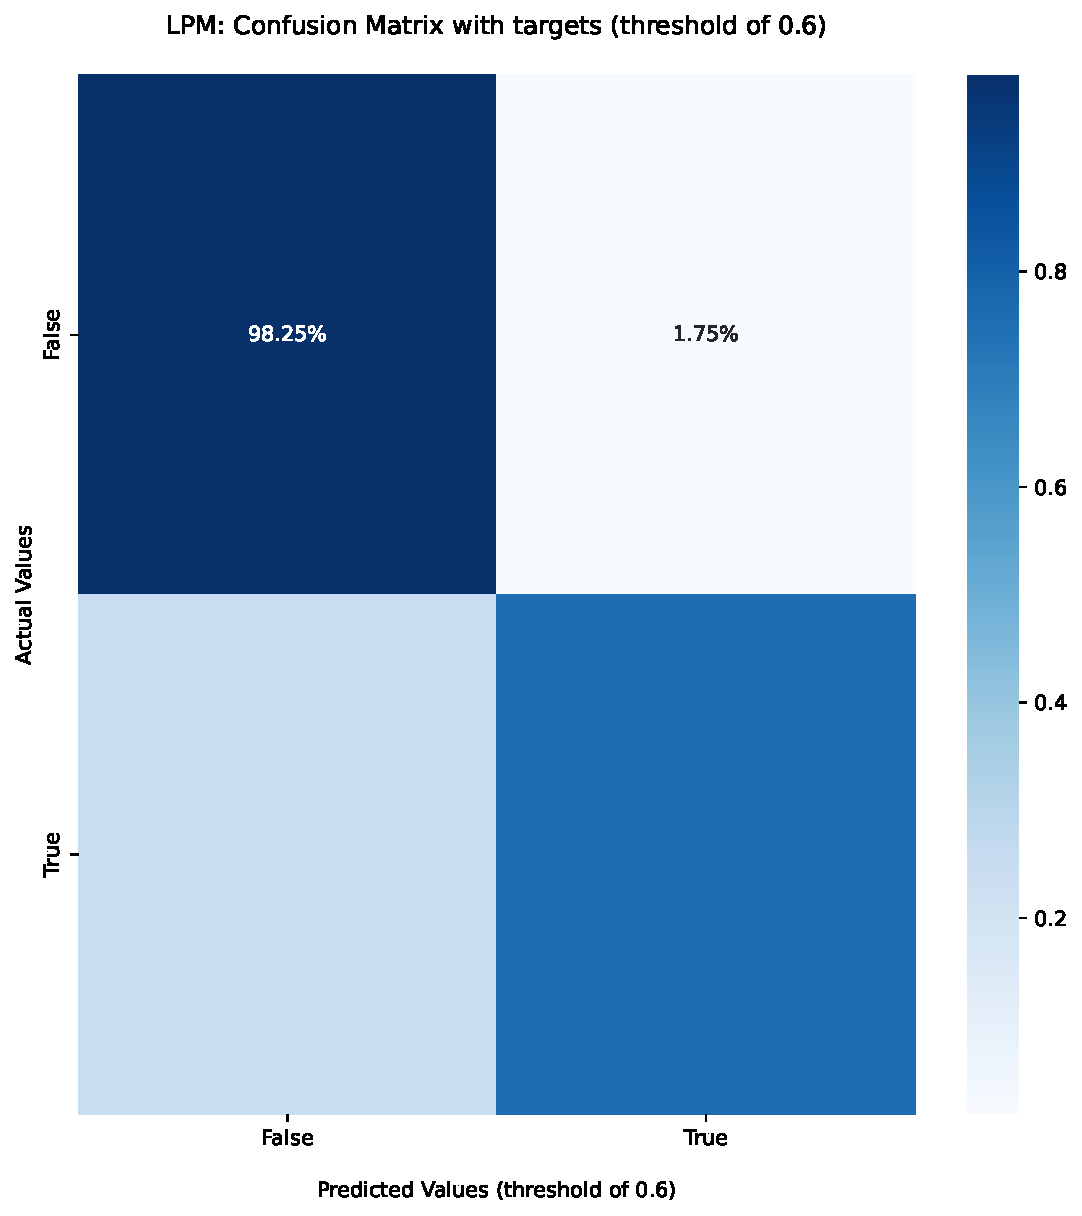
\includegraphics{mp2_files/figure-pdf/cell-8-output-1.pdf}

3.c. Error rate

\begin{Shaded}
\begin{Highlighting}[]
\NormalTok{error\_lpm\_5 }\OperatorTok{=} \DecValTok{1} \OperatorTok{{-}}\NormalTok{ accuracy\_score(target\_valid, lpm\_pred\_5)}
\NormalTok{error\_lpm\_6 }\OperatorTok{=} \DecValTok{1} \OperatorTok{{-}}\NormalTok{ accuracy\_score(target\_valid, lpm\_pred\_6)}

\BuiltInTok{print}\NormalTok{(}\SpecialStringTok{f"The error rate at the 0.5 threshold is approximately: }\SpecialCharTok{\{}\BuiltInTok{round}\NormalTok{(error\_lpm\_5, }\DecValTok{4}\NormalTok{)}\OperatorTok{*}\DecValTok{100}\SpecialCharTok{\}}\SpecialStringTok{\%"}\NormalTok{)}
\BuiltInTok{print}\NormalTok{(}\SpecialStringTok{f"The error rate at the 0.6 threshold is approximately}\SpecialCharTok{\{}\BuiltInTok{round}\NormalTok{(error\_lpm\_6, }\DecValTok{4}\NormalTok{)}\OperatorTok{*}\DecValTok{100}\SpecialCharTok{\}}\SpecialStringTok{\%."}\NormalTok{)}
\end{Highlighting}
\end{Shaded}

\begin{verbatim}
The error rate at the 0.5 threshold is approximately: 9.54%
The error rate at the 0.6 threshold is approximately11.08%.
\end{verbatim}

The 0.5 threshold results in a more accurate prediction.

3.d. Precision = True Positives / (True Positives + False Positives) or
Out of all the positive predictions made, how many are actually
positive? (proportion of positive identifications that were actually
correct)

\begin{Shaded}
\begin{Highlighting}[]
\CommentTok{\# For threshold = 0.5}
\NormalTok{precision\_5 }\OperatorTok{=}\NormalTok{ precision\_score(target\_valid, lpm\_pred\_5, zero\_division}\OperatorTok{=}\DecValTok{0}\NormalTok{)}
\BuiltInTok{print}\NormalTok{(}\SpecialStringTok{f"Positive predictions that were actually correct at the 0.5 threshold: }\SpecialCharTok{\{}\NormalTok{precision\_5}\SpecialCharTok{:.2\%\}}\SpecialStringTok{"}\NormalTok{)}

\CommentTok{\# For threshold = 0.6}
\NormalTok{precision\_6 }\OperatorTok{=}\NormalTok{ precision\_score(target\_valid, lpm\_pred\_6, zero\_division}\OperatorTok{=}\DecValTok{0}\NormalTok{)}
\BuiltInTok{print}\NormalTok{(}\SpecialStringTok{f"Positive predictions that were actually correct at the 0.6 threshold: }\SpecialCharTok{\{}\NormalTok{precision\_6}\SpecialCharTok{:.2\%\}}\SpecialStringTok{"}\NormalTok{)}
\end{Highlighting}
\end{Shaded}

\begin{verbatim}
Positive predictions that were actually correct at the 0.5 threshold: 94.20%
Positive predictions that were actually correct at the 0.6 threshold: 96.77%
\end{verbatim}

3.e.

\begin{Shaded}
\begin{Highlighting}[]
\CommentTok{\# ROC and AUC}
\NormalTok{fpr\_lpm, tpr\_lpm, thresholds\_lpm }\OperatorTok{=}\NormalTok{ roc\_curve(target\_valid, lpm\_pred)}
\NormalTok{auc\_lpm }\OperatorTok{=}\NormalTok{ roc\_auc\_score(target\_valid, lpm\_pred)}

\NormalTok{roc\_curve\_lpm }\OperatorTok{=}\NormalTok{ RocCurveDisplay(}
\NormalTok{fpr}\OperatorTok{=}\NormalTok{fpr\_lpm, tpr}\OperatorTok{=}\NormalTok{tpr\_lpm,}
\NormalTok{roc\_auc}\OperatorTok{=}\NormalTok{auc\_lpm,}
\NormalTok{estimator\_name}\OperatorTok{=}\StringTok{"LPM"}
\NormalTok{)}

\NormalTok{fig, ax }\OperatorTok{=}\NormalTok{ plt.subplots(figsize}\OperatorTok{=}\NormalTok{(}\DecValTok{9}\NormalTok{, }\DecValTok{9}\NormalTok{))}
\NormalTok{roc\_curve\_lpm.plot(ax}\OperatorTok{=}\NormalTok{ax)}
\NormalTok{ax.set\_ylabel(}\StringTok{"True Positive Rate (TPR)"}\NormalTok{, fontsize}\OperatorTok{=}\DecValTok{20}\NormalTok{)}
\NormalTok{ax.set\_xlabel(}\StringTok{"False Positive Rate (FPR)"}\NormalTok{, fontsize}\OperatorTok{=}\DecValTok{20}\NormalTok{)}
\NormalTok{ax.set\_title(}\StringTok{"Receiver Operating Characteristic (ROC) Curve"}\NormalTok{)}
\NormalTok{plt.show()}
\end{Highlighting}
\end{Shaded}

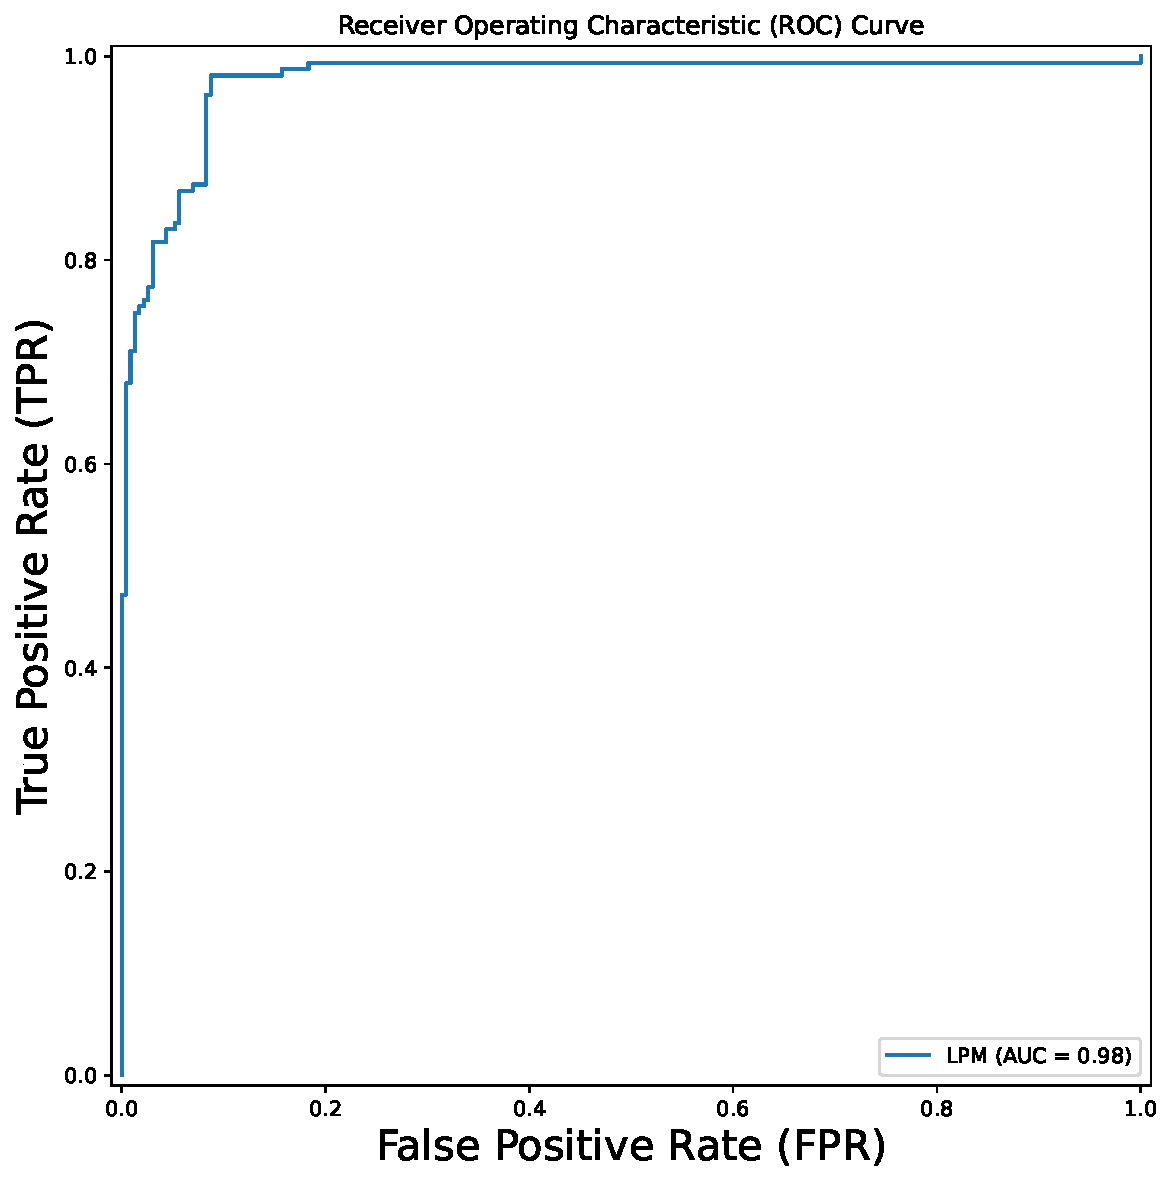
\includegraphics{mp2_files/figure-pdf/cell-11-output-1.pdf}

This curve is closer to the top left corner, which is ideal because we
see a high TPR and a low FPR. This means that the classifier can
correctly identify most positives and has few false positives. This
represents a high level of discrimination capability.

\begin{enumerate}
\def\labelenumi{\arabic{enumi}.}
\setcounter{enumi}{3}
\item
  In measuring performance, policymkaers should care more about
  minimizing false negatives if their priority is ensuring that they are
  able to catch tax evaders. This would mean they should have a lower
  threashold (less FN, higher FP). But if the priority is to not waste
  resources while auditing, then a higher threshold would perform better
  (Min FP, higher FN). We see that there is an inherent trade-off here,
  so government must decide if they want to prioritize curbing tax
  evasion or minimizing their costs.
\item
  KNN for validation set
\end{enumerate}

\begin{Shaded}
\begin{Highlighting}[]
\NormalTok{knn\_5 }\OperatorTok{=}\NormalTok{ KNeighborsClassifier(n\_neighbors}\OperatorTok{=}\DecValTok{5}\NormalTok{)}
\NormalTok{knn\_5.fit(X\_train, target\_train)}
\NormalTok{knn\_5\_pred }\OperatorTok{=}\NormalTok{ knn\_5.predict(X\_valid)}
\end{Highlighting}
\end{Shaded}

5.a.

\begin{Shaded}
\begin{Highlighting}[]
\NormalTok{knn\_cm\_5 }\OperatorTok{=}\NormalTok{ confusion\_matrix(target\_valid, knn\_5\_pred, normalize}\OperatorTok{=}\StringTok{"true"}\NormalTok{)}
\CommentTok{\# Display the visualization of the confusion matrix}
\NormalTok{fig, ax }\OperatorTok{=}\NormalTok{ plt.subplots(figsize}\OperatorTok{=}\NormalTok{(}\DecValTok{9}\NormalTok{, }\DecValTok{9}\NormalTok{))}
\NormalTok{ax }\OperatorTok{=}\NormalTok{ sns.heatmap(}
\NormalTok{knn\_cm\_5, annot}\OperatorTok{=}\VariableTok{True}\NormalTok{, fmt}\OperatorTok{=}\StringTok{".2\%"}\NormalTok{, cmap}\OperatorTok{=}\StringTok{"Blues"}
\NormalTok{)}
\NormalTok{ax.set\_title(}\StringTok{"KNN: Confusion Matrix with targets (k = 5)}\CharTok{\textbackslash{}n}\StringTok{"}\NormalTok{)}
\NormalTok{ax.set\_xlabel(}\StringTok{"}\CharTok{\textbackslash{}n}\StringTok{Predictet Values (threshold = 0.5)"}\NormalTok{)}
\NormalTok{ax.set\_ylabel(}\StringTok{"Actual Values"}\NormalTok{)}
\NormalTok{ax.xaxis.set\_ticklabels([}\StringTok{"False"}\NormalTok{, }\StringTok{"True"}\NormalTok{])}
\NormalTok{ax.yaxis.set\_ticklabels([}\StringTok{"False"}\NormalTok{, }\StringTok{"True"}\NormalTok{])}
\NormalTok{plt.show()}
\end{Highlighting}
\end{Shaded}

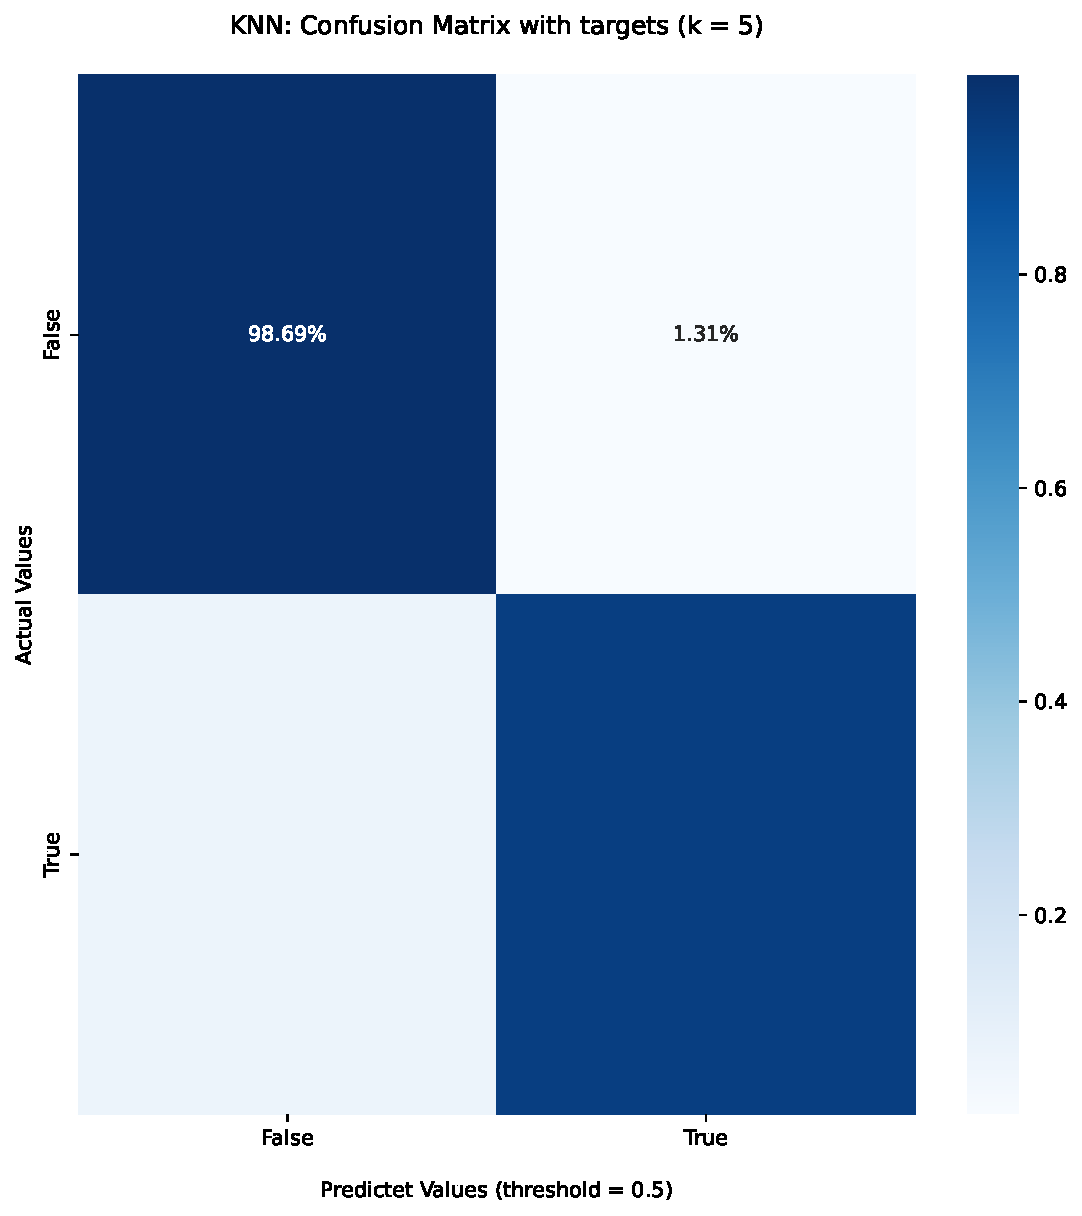
\includegraphics{mp2_files/figure-pdf/cell-13-output-1.pdf}

5.b.Error rate

\begin{Shaded}
\begin{Highlighting}[]
\NormalTok{error\_knn\_5 }\OperatorTok{=} \DecValTok{1} \OperatorTok{{-}}\NormalTok{ accuracy\_score(target\_valid, knn\_5\_pred)}
\BuiltInTok{print}\NormalTok{(}\SpecialStringTok{f"The error rate at the 0.5 threshold for KNN is approximately: }\SpecialCharTok{\{}\BuiltInTok{round}\NormalTok{(error\_knn\_5, }\DecValTok{4}\NormalTok{)}\OperatorTok{*}\DecValTok{100}\SpecialCharTok{\}}\SpecialStringTok{\%"}\NormalTok{)}
\end{Highlighting}
\end{Shaded}

\begin{verbatim}
The error rate at the 0.5 threshold for KNN is approximately: 3.61%
\end{verbatim}

HOW ACCURATE

5.c. Precision

\begin{Shaded}
\begin{Highlighting}[]
\NormalTok{precision\_knn\_5 }\OperatorTok{=}\NormalTok{ precision\_score(target\_valid, knn\_5\_pred, zero\_division}\OperatorTok{=}\DecValTok{0}\NormalTok{)}
\BuiltInTok{print}\NormalTok{(}\SpecialStringTok{f"Positive predictions that were actually correct at the 0.5 threshold: }\SpecialCharTok{\{}\NormalTok{precision\_knn\_5}\SpecialCharTok{:.2\%\}}\SpecialStringTok{"}\NormalTok{)}
\end{Highlighting}
\end{Shaded}

\begin{verbatim}
Positive predictions that were actually correct at the 0.5 threshold: 98.01%
\end{verbatim}

\begin{enumerate}
\def\labelenumi{\arabic{enumi}.}
\setcounter{enumi}{5}
\tightlist
\item
  Scaling
\end{enumerate}

\begin{Shaded}
\begin{Highlighting}[]
\NormalTok{X.dtypes}
\CommentTok{\# we can scale since they are all floats}
\end{Highlighting}
\end{Shaded}

\begin{verbatim}
Sector_score     float64
PARA_A           float64
Risk_A           float64
PARA_B           float64
Risk_B           float64
Money_Value      float64
Risk_D           float64
Score            float64
Inherent_Risk    float64
Audit_Risk       float64
dtype: object
\end{verbatim}

\begin{Shaded}
\begin{Highlighting}[]
\NormalTok{scaler }\OperatorTok{=}\NormalTok{ StandardScaler()  }\CommentTok{\# Initialize the scalar}
\NormalTok{X\_scaled }\OperatorTok{=}\NormalTok{ scaler.fit\_transform(X)  }
\BuiltInTok{print}\NormalTok{(}\BuiltInTok{type}\NormalTok{(X\_scaled)) }
\NormalTok{cols }\OperatorTok{=}\NormalTok{ X.columns  }
\NormalTok{X\_final }\OperatorTok{=}\NormalTok{ pd.DataFrame(X\_scaled, columns}\OperatorTok{=}\NormalTok{cols) }
\NormalTok{X\_final.head()}
\end{Highlighting}
\end{Shaded}

\begin{verbatim}
<class 'numpy.ndarray'>
\end{verbatim}

\begin{longtable}[]{@{}lllllllllll@{}}
\toprule\noalign{}
& Sector\_score & PARA\_A & Risk\_A & PARA\_B & Risk\_B & Money\_Value &
Risk\_D & Score & Inherent\_Risk & Audit\_Risk \\
\midrule\noalign{}
\endhead
\bottomrule\noalign{}
\endlastfoot
0 & -0.669071 & 0.304129 & 0.335827 & -0.166006 & -0.194273 & -0.161614
& -0.190146 & -0.353484 & -0.166753 & -0.141265 \\
1 & -0.669071 & -0.432005 & -0.393216 & -0.119482 & -0.178777 &
-0.198271 & -0.202356 & -0.819385 & -0.276733 & -0.172402 \\
2 & -0.669071 & -0.342190 & -0.363566 & -0.211331 & -0.209370 &
-0.212393 & -0.207059 & -0.819385 & -0.295112 & -0.177606 \\
3 & -0.669071 & -0.432005 & -0.393216 & -0.000278 & 0.004583 & -0.035870
& -0.030676 & 1.976022 & -0.003134 & -0.094940 \\
4 & -0.669071 & -0.432005 & -0.393216 & -0.214326 & -0.210368 &
-0.212393 & -0.207059 & -0.819385 & -0.297523 & -0.178289 \\
\end{longtable}

Now, splitting the data

\begin{Shaded}
\begin{Highlighting}[]
\NormalTok{X\_train, X\_valid, target\_train, target\_valid }\OperatorTok{=}\NormalTok{ train\_test\_split(}
\NormalTok{X\_final, target, train\_size}\OperatorTok{=}\FloatTok{0.50}\NormalTok{, random\_state}\OperatorTok{=}\DecValTok{13}
\NormalTok{)}
\CommentTok{\# Fit the model}
\NormalTok{knn\_5\_scaled }\OperatorTok{=}\NormalTok{ KNeighborsClassifier(n\_neighbors}\OperatorTok{=}\DecValTok{5}\NormalTok{).fit(X\_train, target\_train)}
\CommentTok{\# Apply the model to the validation set}
\NormalTok{knn\_5\_scaled\_pred }\OperatorTok{=}\NormalTok{ knn\_5\_scaled.predict(X\_valid)}
\end{Highlighting}
\end{Shaded}

6.a.

\begin{Shaded}
\begin{Highlighting}[]
\CommentTok{\# Construct confusion matrix}
\NormalTok{knn\_scaled\_cm\_5 }\OperatorTok{=}\NormalTok{ confusion\_matrix(target\_valid, knn\_5\_scaled\_pred, normalize}\OperatorTok{=}\StringTok{"true"}\NormalTok{)}
\CommentTok{\# Display the visualization of the confusion matrix}
\NormalTok{fig, ax }\OperatorTok{=}\NormalTok{ plt.subplots(figsize}\OperatorTok{=}\NormalTok{(}\DecValTok{9}\NormalTok{, }\DecValTok{9}\NormalTok{))}
\NormalTok{ax }\OperatorTok{=}\NormalTok{ sns.heatmap(}
\NormalTok{knn\_scaled\_cm\_5, annot}\OperatorTok{=}\VariableTok{True}\NormalTok{, fmt}\OperatorTok{=}\StringTok{".2\%"}\NormalTok{, cmap}\OperatorTok{=}\StringTok{"Blues"}
\NormalTok{)}
\NormalTok{ax.set\_title(}\StringTok{"KNN (scaled): Confusion Matrix with targets (k = 5)}\CharTok{\textbackslash{}n}\StringTok{"}\NormalTok{)}
\NormalTok{ax.set\_xlabel(}\StringTok{"}\CharTok{\textbackslash{}n}\StringTok{Predictet Values (threshold of 0.5)"}\NormalTok{)}
\NormalTok{ax.set\_ylabel(}\StringTok{"Actual Values"}\NormalTok{)}
\NormalTok{ax.xaxis.set\_ticklabels([}\StringTok{"False"}\NormalTok{, }\StringTok{"True"}\NormalTok{])}
\NormalTok{ax.yaxis.set\_ticklabels([}\StringTok{"False"}\NormalTok{, }\StringTok{"True"}\NormalTok{])}
\NormalTok{plt.show()}
\end{Highlighting}
\end{Shaded}

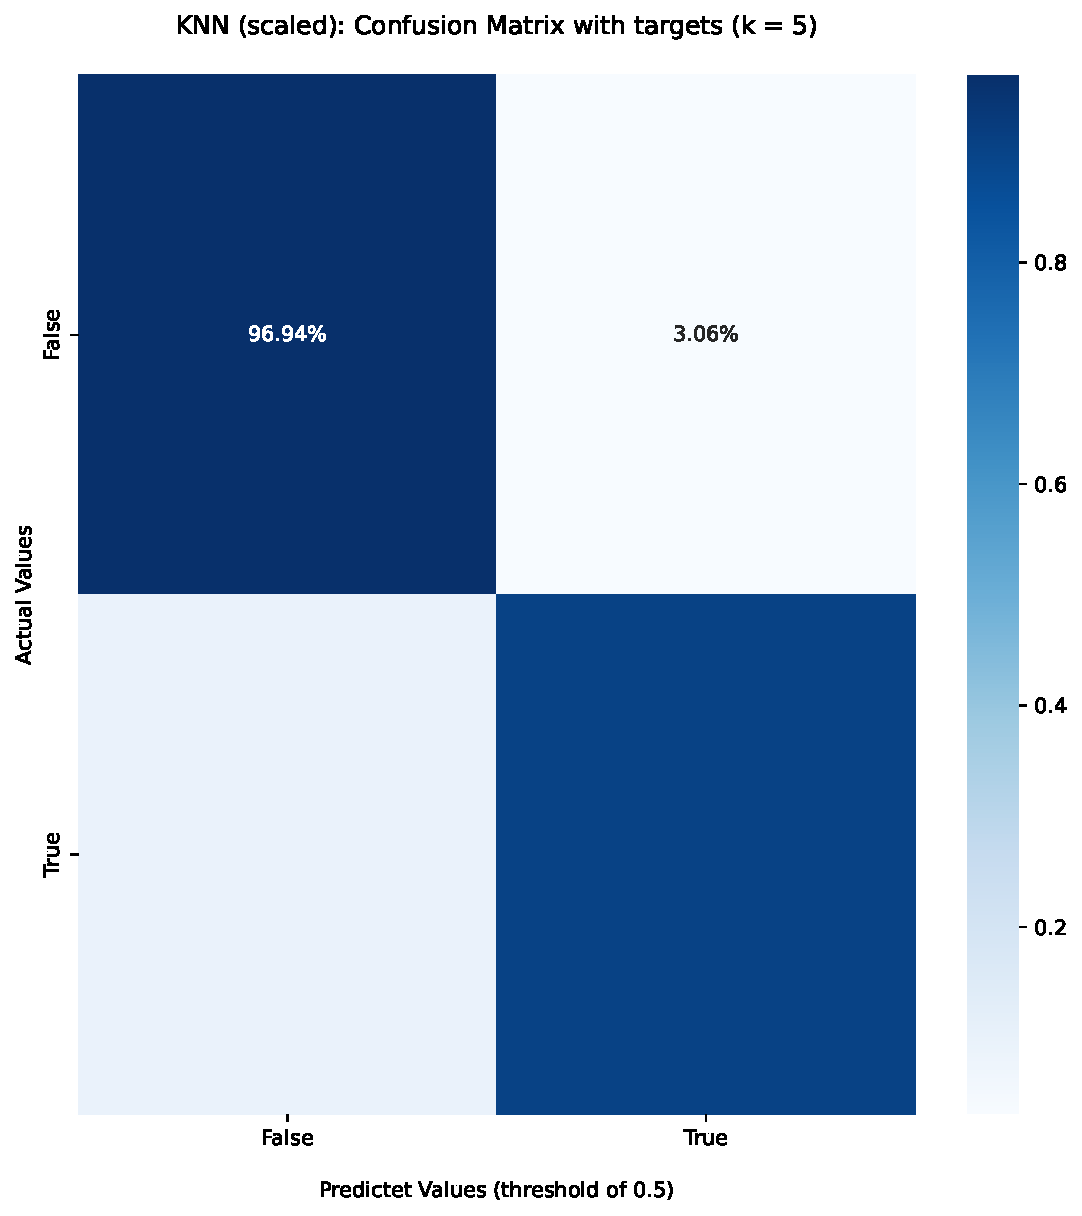
\includegraphics{mp2_files/figure-pdf/cell-19-output-1.pdf}

6.b.

\begin{Shaded}
\begin{Highlighting}[]
\NormalTok{error\_knn\_scaled\_5 }\OperatorTok{=} \DecValTok{1} \OperatorTok{{-}}\NormalTok{ accuracy\_score(target\_valid, knn\_5\_scaled\_pred)}
\BuiltInTok{print}\NormalTok{(}\SpecialStringTok{f"The error rate at the 0.5 threshold for KNN (scaled) is approximately: }\SpecialCharTok{\{}\BuiltInTok{round}\NormalTok{(error\_knn\_scaled\_5, }\DecValTok{4}\NormalTok{)}\OperatorTok{*}\DecValTok{100}\SpecialCharTok{\}}\SpecialStringTok{\%"}\NormalTok{)}
\end{Highlighting}
\end{Shaded}

\begin{verbatim}
The error rate at the 0.5 threshold for KNN (scaled) is approximately: 5.67%
\end{verbatim}

How accurate

6.c.

\begin{Shaded}
\begin{Highlighting}[]
\NormalTok{precision\_knn\_scaled\_5 }\OperatorTok{=}\NormalTok{ precision\_score(target\_valid, knn\_5\_scaled\_pred, zero\_division}\OperatorTok{=}\DecValTok{0}\NormalTok{)}
\BuiltInTok{print}\NormalTok{(}\SpecialStringTok{f"Positive predictions that were actually correct at the 0.5 threshold: }\SpecialCharTok{\{}\NormalTok{precision\_knn\_scaled\_5}\SpecialCharTok{:.2\%\}}\SpecialStringTok{"}
\NormalTok{)}
\end{Highlighting}
\end{Shaded}

\begin{verbatim}
Positive predictions that were actually correct at the 0.5 threshold: 95.36%
\end{verbatim}

\begin{enumerate}
\def\labelenumi{\arabic{enumi}.}
\setcounter{enumi}{6}
\item
  The non-normalized KNN model appears to perform better in this case
  (Error rate is 3.61\%, Precision is 98.01\%) compared to the
  normalized one (Error rate is 5.67\%, Precision is 95.36\%). This is
  somewhat unexpected, as normalization usually improves KNN
  performance. Maybe the original scale of the features already captures
  important information about their relative importance.
\item
  For KNN, which k yields the lowest error rate? By 5-fold
  cross-validation (5FCV), find the k with the lowest classification
  error rate. Briefly explain. 6Use the entire dataset for 5FCV, shuffle
  the data randomly for splitting, and set random\_state=13
\end{enumerate}

\begin{Shaded}
\begin{Highlighting}[]
\ImportTok{from}\NormalTok{ sklearn.model\_selection }\ImportTok{import}\NormalTok{ GridSearchCV, KFold}
\ImportTok{from}\NormalTok{ sklearn.neighbors }\ImportTok{import}\NormalTok{ KNeighborsClassifier}

\CommentTok{\#\# Re{-}split data so it is not normalized }
\NormalTok{X\_train, X\_valid, target\_train, target\_valid }\OperatorTok{=}\NormalTok{ train\_test\_split(}
\NormalTok{X, target, train\_size}\OperatorTok{=}\FloatTok{0.50}\NormalTok{, random\_state}\OperatorTok{=}\DecValTok{13}
\NormalTok{)}


\CommentTok{\# Select a range of KNN neighbors (k) to evaluate}
\NormalTok{ks }\OperatorTok{=} \BuiltInTok{list}\NormalTok{(}\BuiltInTok{range}\NormalTok{(}\DecValTok{1}\NormalTok{, }\DecValTok{37}\NormalTok{, }\DecValTok{2}\NormalTok{))}
\NormalTok{param\_grid }\OperatorTok{=}\NormalTok{ \{}\StringTok{\textquotesingle{}n\_neighbors\textquotesingle{}}\NormalTok{: ks\}}

\CommentTok{\# Initialize the KNN classifier}
\NormalTok{knn }\OperatorTok{=}\NormalTok{ KNeighborsClassifier()}

\CommentTok{\# Set up 5{-}fold cross{-}validation scheme}
\NormalTok{kfcv }\OperatorTok{=}\NormalTok{ KFold(}\DecValTok{5}\NormalTok{, random\_state}\OperatorTok{=}\DecValTok{13}\NormalTok{, shuffle}\OperatorTok{=}\VariableTok{True}\NormalTok{)}

\CommentTok{\# Perform GridSearchCV}
\NormalTok{knn\_cv }\OperatorTok{=}\NormalTok{ GridSearchCV(knn, param\_grid, cv}\OperatorTok{=}\NormalTok{kfcv)}
\NormalTok{knn\_cv.fit(X\_train, target\_train)}
\NormalTok{knn\_cv\_pred }\OperatorTok{=}\NormalTok{ knn\_cv.predict(X\_valid)}
\NormalTok{knn\_cv\_pred\_acc }\OperatorTok{=}\NormalTok{ accuracy\_score(target\_valid, knn\_cv\_pred)}
\CommentTok{\# Get the best k and its corresponding score}
\NormalTok{best\_k }\OperatorTok{=}\NormalTok{ knn\_cv.best\_params\_[}\StringTok{\textquotesingle{}n\_neighbors\textquotesingle{}}\NormalTok{]}
\NormalTok{best\_score }\OperatorTok{=}\NormalTok{ knn\_cv.best\_score\_}

\BuiltInTok{print}\NormalTok{(}\StringTok{"Best parameters:"}\NormalTok{, knn\_cv.best\_params\_)}
\BuiltInTok{print}\NormalTok{(}\StringTok{"Best cross{-}validation score:"}\NormalTok{, knn\_cv.best\_score\_)}
\BuiltInTok{print}\NormalTok{(}\StringTok{"Accuracy Score:"}\NormalTok{, knn\_cv\_pred\_acc)}




\CommentTok{\# Plot the results}
\NormalTok{plt.figure(figsize}\OperatorTok{=}\NormalTok{(}\DecValTok{10}\NormalTok{, }\DecValTok{6}\NormalTok{))}
\NormalTok{plt.plot(ks, knn\_cv.cv\_results\_[}\StringTok{\textquotesingle{}mean\_test\_score\textquotesingle{}}\NormalTok{])}
\NormalTok{plt.xlabel(}\StringTok{\textquotesingle{}Number of Neighbors (k)\textquotesingle{}}\NormalTok{)}
\NormalTok{plt.ylabel(}\StringTok{\textquotesingle{}Cross{-}validation Accuracy\textquotesingle{}}\NormalTok{)}
\NormalTok{plt.title(}\StringTok{\textquotesingle{}KNN: Accuracy vs. k\textquotesingle{}}\NormalTok{)}
\NormalTok{plt.show()}
\end{Highlighting}
\end{Shaded}

\begin{verbatim}
Best parameters: {'n_neighbors': 1}
Best cross-validation score: 0.9638694638694638
Accuracy Score: 0.9587628865979382
\end{verbatim}

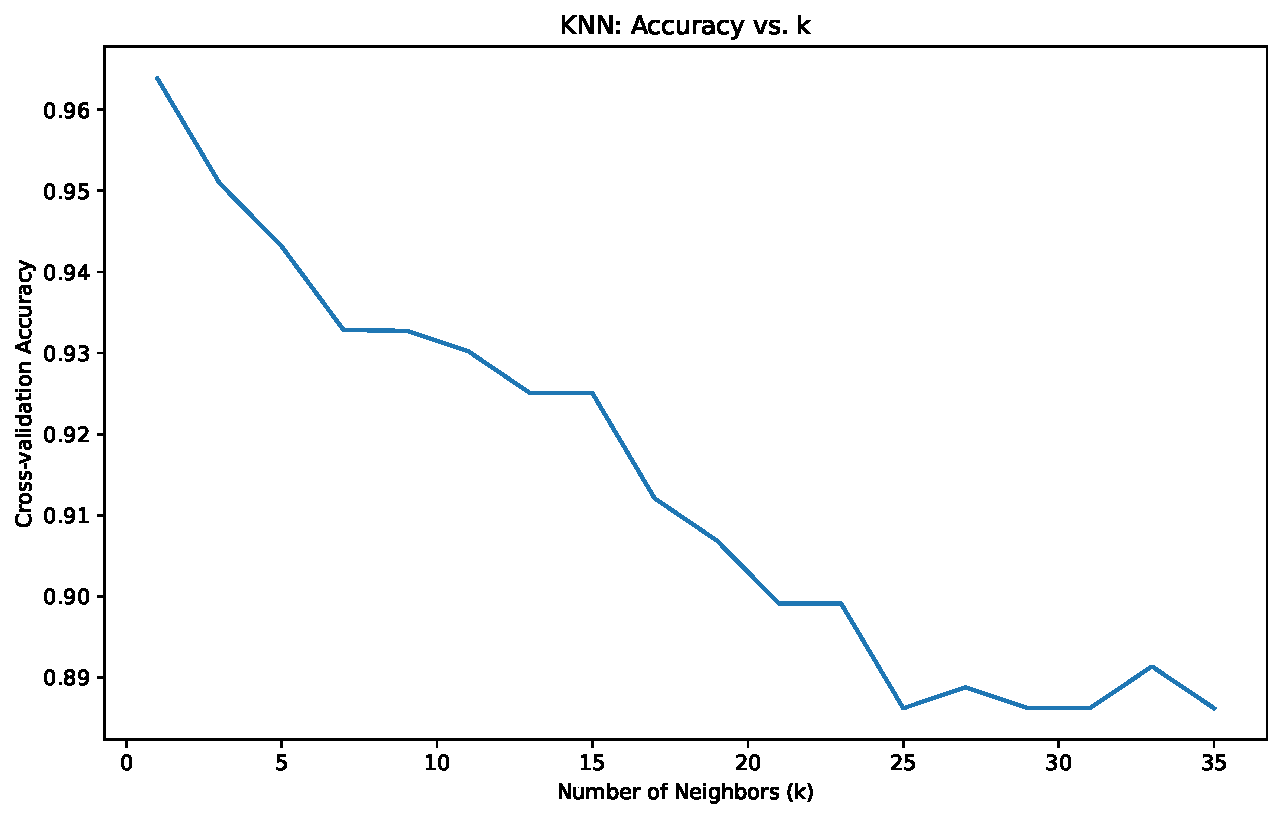
\includegraphics{mp2_files/figure-pdf/cell-22-output-2.pdf}

The optimal k for KNN using the 5FCV is k=1 because it gives us the best
cross-validation score of approximately 96.39\% and an accuracy score of
95.88\% on the validation set. It is highly flexible since each
observation is classified based solely on a single nearest neighbor.
This can lead to low bias but potentially high variance. Since this
flexible model is complex, it is likely that the relationship between
the predictors and the dependent variable, RISK, is a complex one.

\begin{enumerate}
\def\labelenumi{\arabic{enumi}.}
\setcounter{enumi}{8}
\tightlist
\item
  Since the dataset only contains firms that were audited, we mmay run
  into the problem of selection bias. We are looking at firms who we
  already suspected of foul play, so the model doesn't really capture
  the entire population of firms. In the long run, the model may not
  detect new patterns of tax evasion for unaudited firms and instead
  overfit on characteristics of firms that are in the data/audited. To
  deal with this, the government should regularly feed the model with
  new data and this time do a random sampling so that we can avoid the
  bias. Finally, we should make sure to regularly evaluate the model's
  performance.
\end{enumerate}




\end{document}
